\chapter{Database Schema}
\label{ch:database-schema}

\section{Schema Overview}
\label{sec:schema-overview}

This chapter provides the complete SQL schema definition for \projectname{}, including all tables, columns, data types, constraints, and indexes.

% ============================================
% SCHEMA DIAGRAM
% ============================================
\section{Visual Schema Diagram}
\label{sec:schema-diagram}

\begin{figure}[H]
\centering
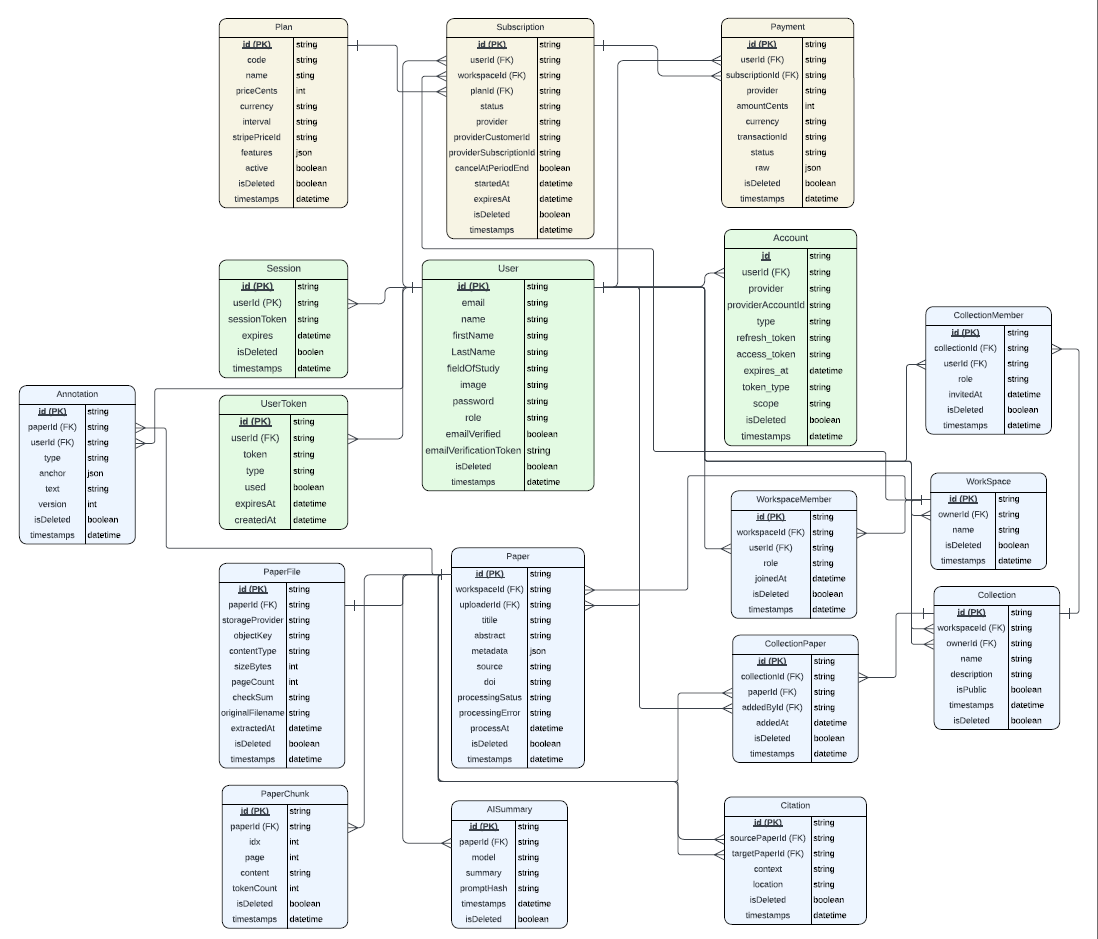
\includegraphics[width=0.95\textwidth]{images/diagrams/schema.png}
\caption{ScholarFlow Complete Database Schema}
\label{fig:schema-complete}
\end{figure}

\noindent For detailed schema view: \url{https://lucid.app/lucidchart/8fa45201-ebc1-46e2-8204-93c162cbaf0b}

% ============================================
% TABLE DEFINITIONS
% ============================================
\section{Core Table Definitions}
\label{sec:schema-tables}

\subsection{User Table}

\begin{lstlisting}[language=SQL, caption={User Table Schema}]
CREATE TABLE "User" (
  id SERIAL PRIMARY KEY,
  name VARCHAR(255),
  email VARCHAR(255) UNIQUE NOT NULL,
  emailVerified TIMESTAMP,
  image TEXT,
  password TEXT,
  role VARCHAR(50) DEFAULT 'RESEARCHER',
  bio TEXT,
  institution VARCHAR(255),
  field VARCHAR(255),
  googleScholarUrl TEXT,
  orcidUrl TEXT,
  createdAt TIMESTAMP DEFAULT NOW(),
  updatedAt TIMESTAMP DEFAULT NOW()
);

-- Indexes
CREATE UNIQUE INDEX "User_email_key" ON "User"(email);
CREATE INDEX "User_role_idx" ON "User"(role);
\end{lstlisting}

\subsection{Paper Table}

\begin{lstlisting}[language=SQL, caption={Paper Table Schema}]
CREATE TABLE "Paper" (
  id SERIAL PRIMARY KEY,
  title VARCHAR(500) NOT NULL,
  authors TEXT,
  abstract TEXT,
  publicationYear INTEGER,
  journal VARCHAR(255),
  doi VARCHAR(255),
  fileUrl TEXT NOT NULL,
  fileName VARCHAR(500) NOT NULL,
  fileSize BIGINT NOT NULL,
  fileType VARCHAR(50) NOT NULL,
  uploaderId INTEGER NOT NULL REFERENCES "User"(id),
  workspaceId INTEGER NOT NULL REFERENCES "Workspace"(id),
  isDeleted BOOLEAN DEFAULT FALSE,
  deletedAt TIMESTAMP,
  createdAt TIMESTAMP DEFAULT NOW(),
  updatedAt TIMESTAMP DEFAULT NOW()
);

-- Performance Indexes
CREATE INDEX "Paper_uploaderId_workspaceId_idx" 
  ON "Paper"(uploaderId, workspaceId);
CREATE INDEX "Paper_workspaceId_isDeleted_idx" 
  ON "Paper"(workspaceId, isDeleted);
CREATE INDEX "Paper_title_authors_gin_idx" 
  ON "Paper" USING gin(to_tsvector('english', title || ' ' || authors));
\end{lstlisting}

% NOTE: Additional tables should be added here
% See apps/backend/prisma/schema.prisma for complete definitions
% Key tables to include:
% - Workspace
% - Collection
% - AISummary
% - Subscription
% - Annotation
% - CitationExport
% etc.

\section{Complete Schema SQL}
\label{sec:schema-complete-sql}

\begin{infobox}[Full Schema]
The complete schema includes 24 tables with all relationships. For the full Prisma schema definition, see:

\texttt{apps/backend/prisma/schema.prisma}

Or generate SQL:
\begin{lstlisting}[language=bash]
yarn db:migrate dev --name schema_export
\end{lstlisting}
\end{infobox}
